\documentclass{article}

\usepackage{booktabs}
\usepackage{float}
\usepackage{graphicx}

\author{Michael Davis 	\\
		Maxwell Peterson \\
		Robert Sheehy 	\\
		Mark Gollnick 	\\
		Taehyun Park	}
		
\title{Web Tournaments \\
	   Final Report}
		
\begin{document}
\maketitle



\newpage
\section{Introduction}

\subsection{Purpose}
The purpose of this document is to enumerate and elaborate on the requirements and design of the Web Tournaments web application. This document should enable the reader to understand the thought process of the programmers as they put together the different components of the project.

\subsection{Scope}
The project aims to solve the problems presented when keeping track of tournaments on paper and white boards. There is a lot of manual work and logic involved when doing tournaments the old fashioned way, such as calculating seeds after a round robin or trying to draw a double elimination bracket for 17 people. The goal of this project is to create a platform on the web that can handle many different kinds of tournaments. A platform that will eventually be expanded upon, but for the purposes of this project we will only implement a few kinds of tournaments due to time constraints. The plan for this project is to fully implement single and double elimination tournaments, as well as round robin tournaments. If there is time we would like to be able to calculate seeds from round robin results to go into a single or double elimination bracket.

\subsection{Definitions, Acronyms, Abbreviations}
\begin{table}[h]
	\centering
	\begin{tabular}{p{3cm} p{8cm}}
		\toprule
		Term & Description  \\

		\midrule

		Round Robin Tournament & A type of tournament in which each player or team plays every other player or team in the tournament or pool. 		\\
		\midrule
		Single Elimination Tournament & A type of tournament in which a player or team can only lose once before they are out of the tournament.	\\
		\midrule
		Double Elimination Tournament & A type of tournament in which a player or team can lose twice before being out of the tournament. After losing once, they enter the consolation bracket, which at best can win third place.	\\

		\bottomrule
	\end{tabular}
\end{table}

\newpage
\subsection{Design Goals}
\subsubsection{Usability}
The end product should be easy to use, and intuitive. It should not require an instruction manual or help pages to use. The user should not be confused about what to do next, and it should have a kind of ‘flow’ of easiness.

\subsubsection{Extensibility}
The project should be able to be expanded upon after the semester has ended. New tournament types and user interface interactions should easily be able to be added and modified.

\subsubsection{Reliability}
Having a reliable and working copy of the code at all times is top priority.  In order make the application as reliable as possible, all code must be reviewed by one other person on the team before making it into master.  Github makes this easy with the pull request functionality.  At all times master is production quality code and could be pushed to production at any time. 

\subsubsection{Quick and easy tournament creation}
Creating a user’s first tournament should not require logging in until after they have gone through the tournament creation wizard.  After the tournament has been created, the user should have the option to create and account and be able to take ownership of the tournament that they have already created.  

\subsubsection{Response Time}
The service should respond quickly when an action is performed. No page should take more than 3 full seconds to load (internet connection not being the limiting factor)



\newpage
\section{References}
\subsection{Google App Engine}
Free/Low cost hosting solution that is able to quickly scale with our app and has the power of Google behind it.

\subsection{Flask}
A slim web application framework for Python. Our team discovered this as a replacement for webapp2 and thought it looked really nice. This framework handles HTTP requests and routing based on URL patterns.

\subsection{WTForms}
The forms library. It allows developers to create a form class with field attributes which end up being rendered into HTML forms easily.

\subsection{Jinja Templates}
The HTML templating language. Create HTML templates with variables passed into them; ability to do loops and template subclassing/extension.

\subsection{Flask extensions}
Various flask extensions are used such as flask-login, flask-oauth, and flask- assets.

\subsection{Twitter Bootstrap}
An awesome frontend framework that provides us with a slick look and feel for the web application, without having a graphic designer on the team.

\subsection{jQuery}
Making javascript not horrible since 2006. It helped with making AJAX calls and refreshing things on the page.

\subsection{jQuery Datatables}
Easily making searchable and sortable tables.

\subsection{Github}
Github allows for us to take advantage of a large number of code management tools.  Code reviews on every single pull request.  Easy branching.  Excellent code tracking. 

\subsection{Trello}
Trello is a task tracker built around an agile workflow.  There are a number of swimming lanes that tickets can advance to in their path to being completed.  This helps us to quickly see that status of all items that are in progress. 

\subsection{Agile software development}
Weekly sprints allow us to easily keep tabs on everything that is going on with the team, and have a good understanding of every member's progress with their work.  This also helped with motivation, as each team member had to present their progress every week.


\newpage
\section{User Interface Description}
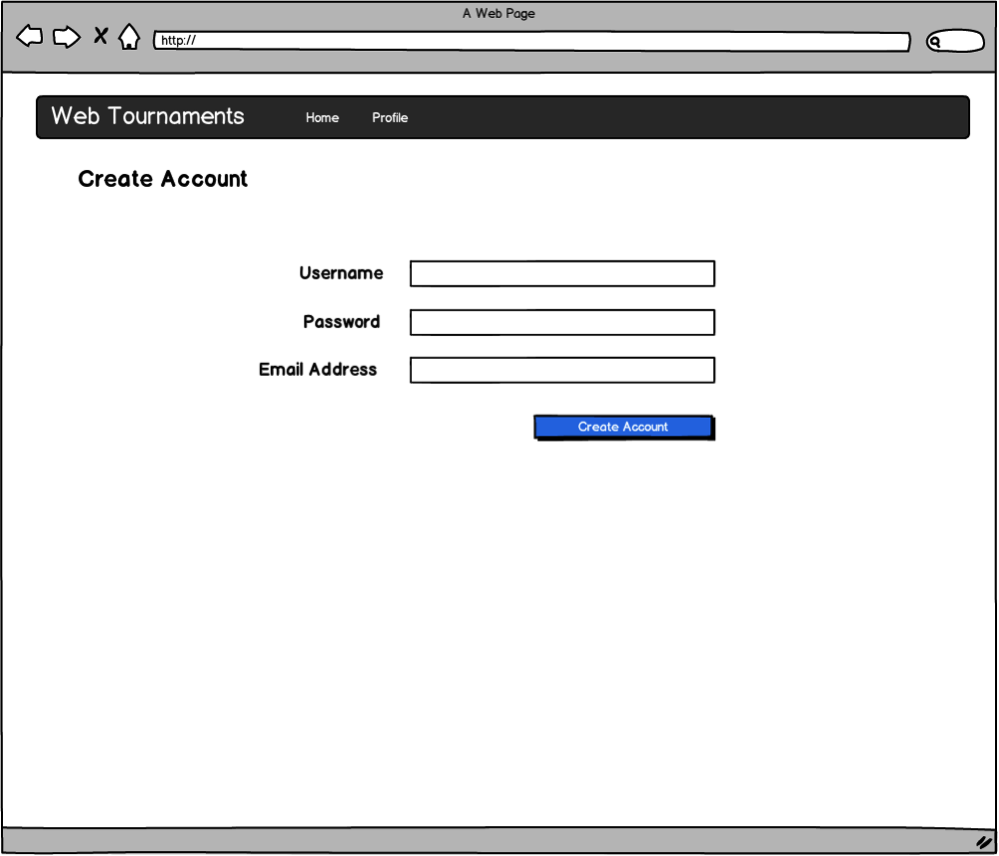
\includegraphics[width=1\textwidth]{one}
\newpage
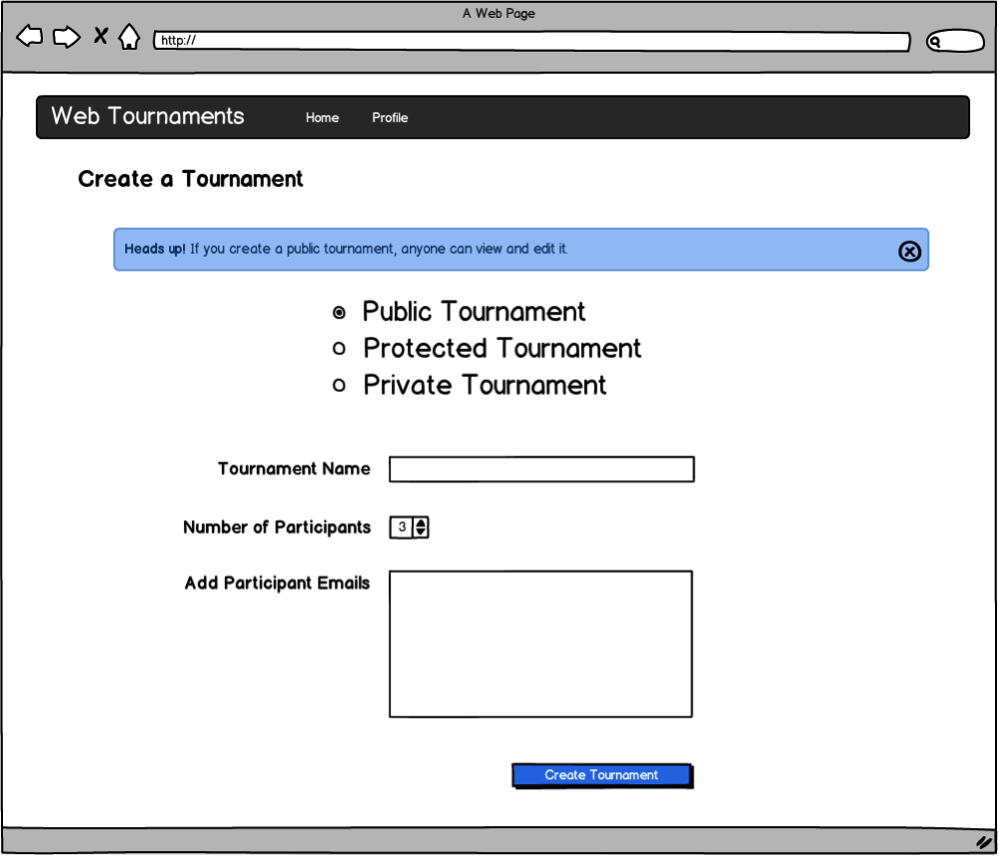
\includegraphics[width=1\textwidth]{two}
\newpage
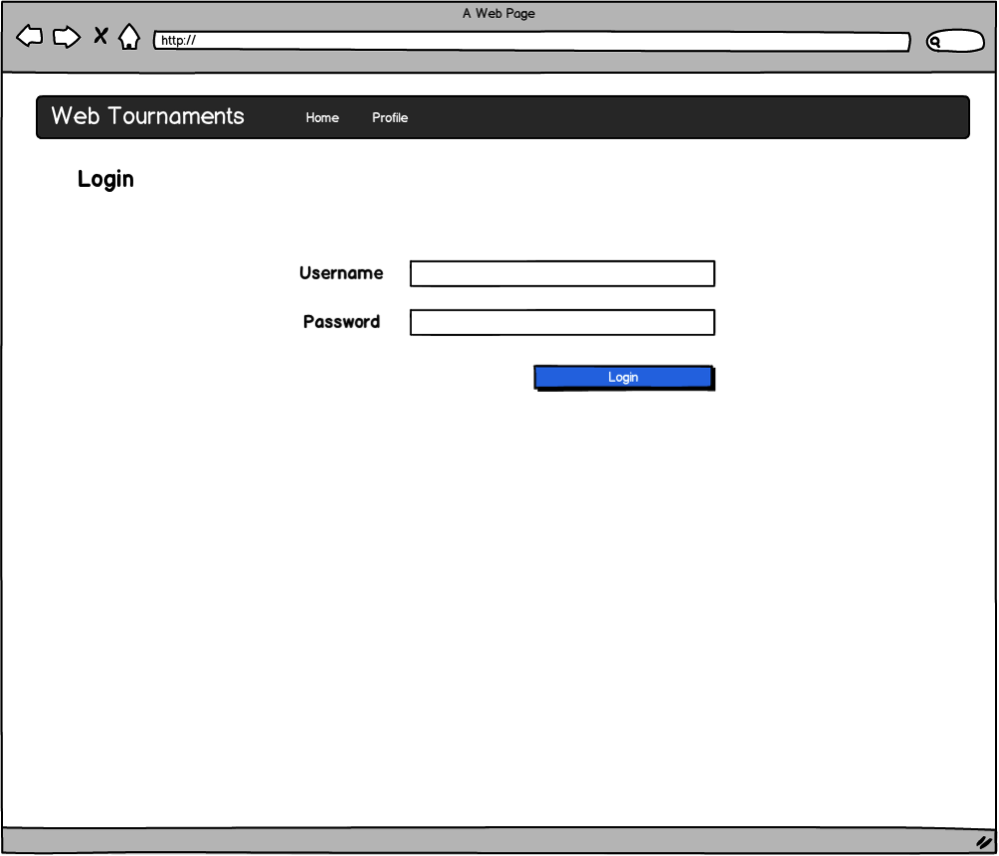
\includegraphics[width=1\textwidth]{three}
\newpage
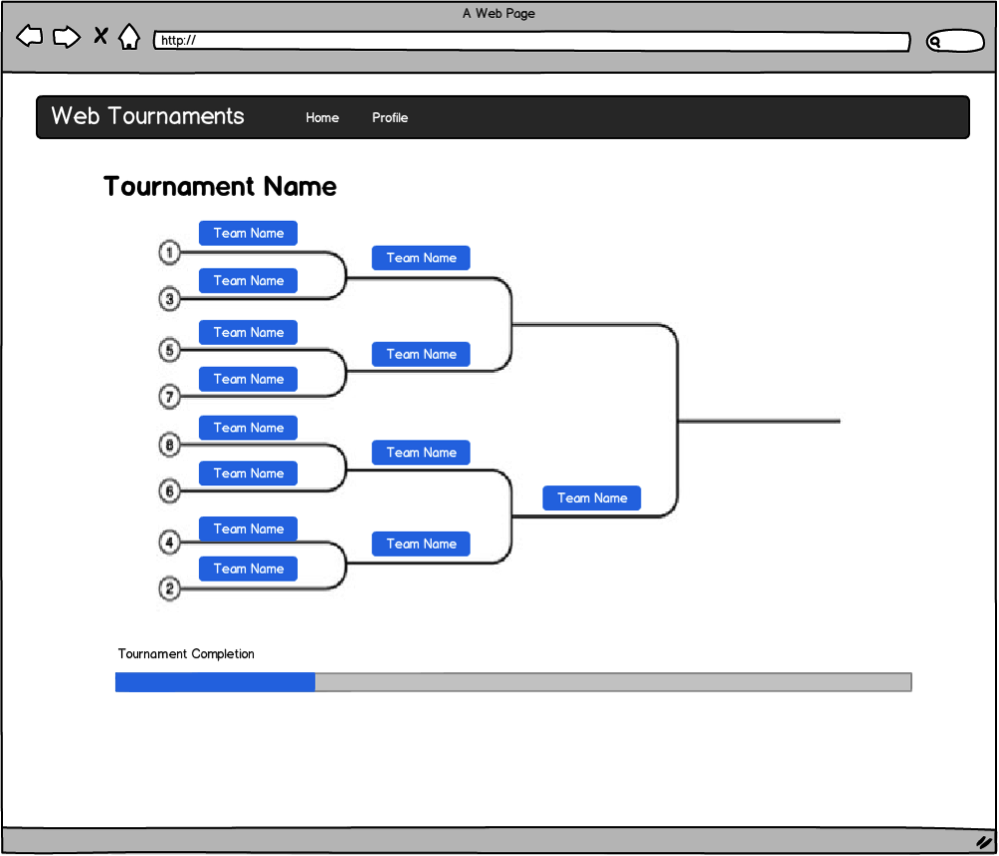
\includegraphics[width=1\textwidth]{four}
\newpage
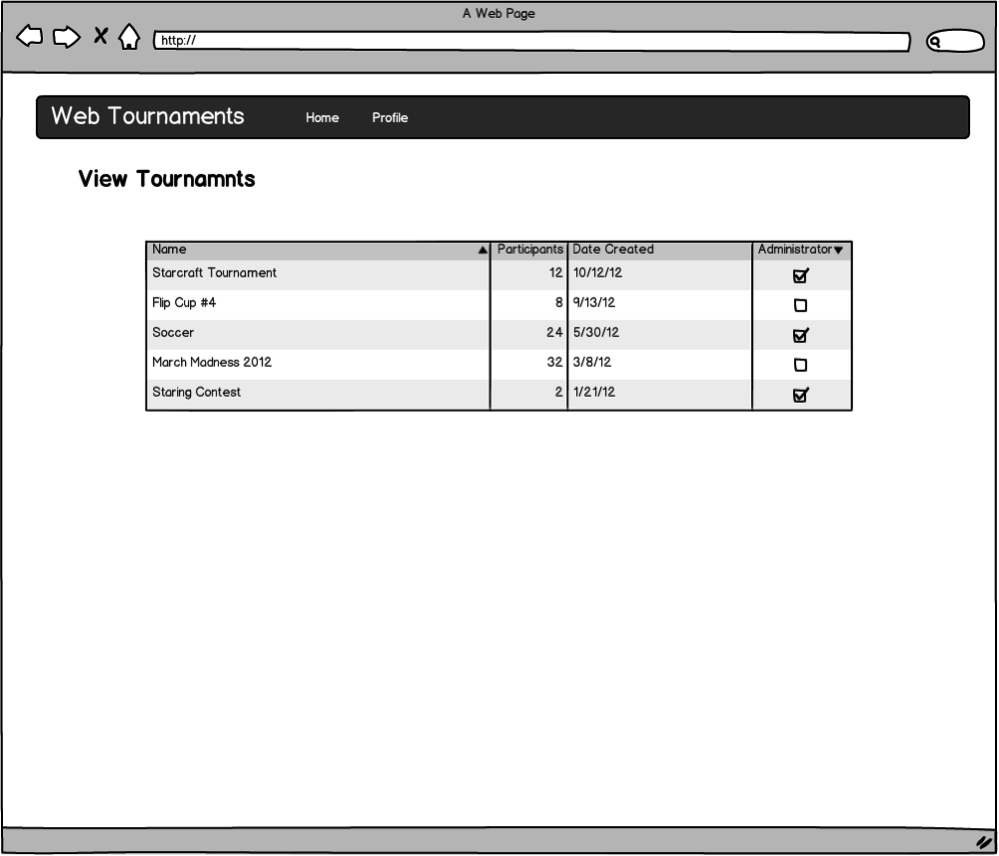
\includegraphics[width=1\textwidth]{five}



\newpage
\section{Decomposition Diagram}

\subsection{Module Decomposition}
Modules are broken up by topic area. Each module contains classes that describe anything needed for that topic area. There are classes for forms, models, views, utilities, and different database actions that pertain to each module. For example, checking a password as valid would be found in the utilities section of the auth module.

\subsubsection{Auth}
The auth module includes a number of methods for dealing with user creation, authentication, and management. It includes the model descriptions for users, form descriptions for the register and login forms, and utilities for generating password hashes, generating secure tokens, validating tokens, and other authentication related tasks. All of the logic for validating a login and handling a user session is also included.

\subsubsection{Base}
The base module includes the methods and utilities that didn’t fit in any of the other modules. It includes mail functionality and form widgets that are used across the entire app.

\subsubsection{Lib}
Lib houses all of our external libraries needed to run the application.

\subsubsection{Tournament}
The tournament module houses all of the forms, models, utilities, database actions, and views for all of the tournament functionality. Actions houses all of the database interaction such as creating a tournament, updating a tournament, and getting tournament information out of the database. Forms contains all of the forms needed for dealing with tournaments, including the forms needed to create, edit and delete a tournament and the forms needed to update a tournament from the tournament view page. Models contains all of the model descriptions for our tournaments, including the models for Tournaments, Matches, and Tournaments. This module has grown to be quite large, and should really be split into multiple modules at this point.

\newpage
\subsection{Concurrent Processes}
Our application does not currently use multiple threads. Google App Engine provides minimal support for multi-threaded applications.  In the future there are plans for using task queues for creating large tournaments, but it has not been implemented at this point.

\subsection{Data Decomposition}
\subsubsection{WTUser}
The WTUser module stores the information about different users. It includes properties that include username, email, salt, password, and Facebook or Google identifiers used in OAuth authentication.

\subsubsection{Tournament}
The Tournament model contains information about a complete tournament. This includes information such as the name, type, date, and location of the tournament, along with permissions on the tournament.

\subsubsection{Match}
The Match model contains information about a specific match in a tournament. It includes information such as the round of the tournament it is in, if it has been played, and contains a reference to the next match that the winner should advance to in a bracket tournament.

\subsubsection{Participant}
The Participant model contains information about one player in a specific match. It includes information about the player such as seed, a reference to a user, and a name field.

\subsection{Overall System Specification}
N/A – Our application does not live on a typical server system, but instead on the Google App Engine platform.



\newpage
\section{Dependency Description}
\subsection{Intermodule Dependencies}
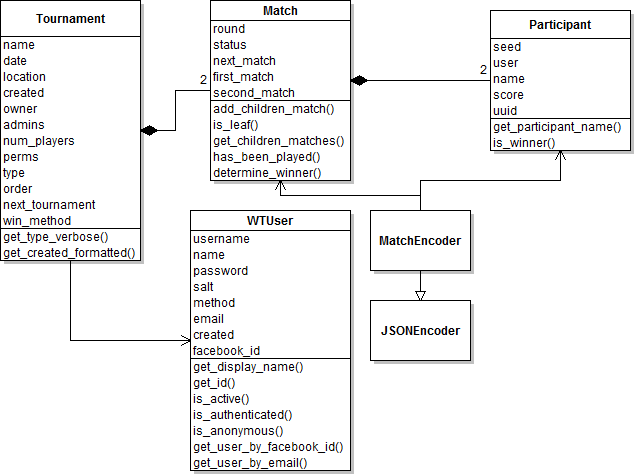
\includegraphics[width=1\textwidth]{intermodule}

\newpage
\subsection{Interprocess Dependencies}
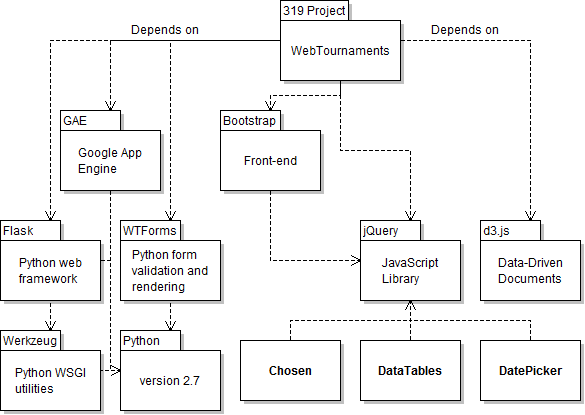
\includegraphics[width=1\textwidth]{interprocess}

\subsection{Data Dependencies}
The user and tournament data is stored in the datastore, which is a non- relational database managed and scaled by Google App Engine. When Displaying a tournament bracket, the data is requested at a designated endpoint using the tournament’s ID key, where it is then translated from Python objects into a JSON representation.



\newpage
\section{Interface Description}
\subsection{Module Interface}
\subsubsection{Views Module}
Included in Auth and Tournament modules.  This handles the logic behind getting the required information for the html template to display to the user. 
\subsubsection{Register(request)}
Handles the logic dealing with registering a new user.
\subsubsection{Login(request)}
Handles the logic dealing with logging a user in
\subsubsection{New\_Tournament(request)}
Handles the logic in creating a new tournament.
\subsubsection{Tournament\_Edit(request, tournament\_key)}
Handles the logic to edit a tournament.  Takes a tournament key of the tournament to edit. 
\subsubsection{Tournament\_View(request, tournament\_key)}
Handles the logic to view a a tournament.  Takes a tournament key of the tournament to edit.
\subsubsection{Tournament\_Search(request)}
Handles the logic with searching for tournaments.
\subsubsection{Actions Module}
Handles all of the access to the database and extends those functions to other modules. 
\subsection{Process Interface}
N/A



\newpage
\section{Design Issues}
\subsection{Tournament Visualization with D3.js}
\subsubsection{Description}
Displaying tournament brackets of single elimination was difficult. We hoped to find a framework that it uses in order to display nodes.

\subsubsection{Factors affecting Issue}
Until we figured out how to use D3 properly, we could not display tournaments. It affected us by not allowing use to demo the project significantly during the checkpoint.

\subsubsection{Alternatives and their pros and cons}
We considered using gRapheal before we discovered D3, but it proved to be too limited for our uses. gRapheal is geared more for the creation of charts rather than graphs. Aside from this limitation, D3 and gRapheal have similar jQuery-like interaction, which is a positive.

\subsubsection{Resolution of Issue}
We discovered D3.js and it allowed us to have the functionality that we needed in order draw brackets on the screen in an acceptable way.

\subsection{Tournament Generation Algorithm}
\subsubsection{Description}
Creating a tournament with an odd number of participants does not work properly.

\subsubsection{Factors affecting Issue}
The complexity of the algorithm took us a while to figure out. Our first approach towards creating a single elimination tournament was to create matches from the bottom to top recursively. Since there was no way to traverse or get the children of a parent node with the initial match model, we revised it to have children nodes, left\_match and right\_match. With the revised match model, we could create matches and connect them from top to bottom.

\subsubsection{Alternatives and their pros and cons}
Running time of the algorithm did not make a difference because bot algorithm occur in O(n) time. The only downside of the new algorithm is that it uses more space in the database to store the keys of the left and right matches, but that is very minimal.

\subsubsection{Resolution of Issue}
We revised, and continue to revise, the model and algorithm.



\newpage
\section{Tracability}
\begin{table}[h]
	\centering
	\begin{tabular}{lll}
		\toprule
		No & Use Case & Subsystem that handles it \\
		\midrule
		1 & User Creation & Auth 					\\
		\midrule
		2 & User Login & Auth 					\\
		\midrule
		3 & Tournament Creation & Tournament 		\\
		\midrule
		4 & Tournament Updating & Tournament 		\\
		\midrule
		5 & Link User to Tournament & Tournament  \\
		\bottomrule
	\end{tabular}
\end{table}



\newpage
\section{Languages and Frameworks}
\subsection{Python}
We love Python. It is especially good for writing web applications due to its simple syntax and high-level approach at programming. When writing code for a web application we are not concerned with the extreme performance or the low level access of memory (pointers, bit- shifting) of a language like C. Instead Python lets us focus on the logic of the application and helps us complete the task in fewer lines of code.

\subsection{Flask}
This was the first time that any of us had used the flask micro-framework. We had originally planned on using webapp2, and even started coding the skeleton of the application on it. But then we discovered Flask. Flask is similar to webapp2, but has far better documentation and community involvement. We were able to find some useful flask plugins (like flask-oauth) that simply do not exist for webapp2. Some of us had a lot of prior experience with Django, a larger Python web-application framework. But Django is big and sluggish compared to the slim flask framework. We enjoyed learning how to leverage flask and many of us will probably use flask again for our next Python web application.

\subsection{Google App Engine}
Our application is served by a scalable cloud-based web application hosting service called Google AppEngine. AppEngine runs web applications written in Java, Python, or Go languages. It supplies a scalable non-relational database called BigTable, where all of our data gets stored. AppEngine applications have a free daily quota, which is perfect for school projects like this one. As long as your application doesn’t use up a lot of instance hours or database storage, it won’t cost a dime. Of course if it ever begins to be widely used, we can begin paying for resources.

\subsection{Javascript/jQuery/d3}
A lot of the frontend interactions are written in javascript and jQuery. We make use of AJAX calls to send updated match scores using JSON. jQuery makes constructing AJAX calls as easy as possible: simply provide a URL endpoint and some JSON to send, and a function to call when it gets a response. We also make use of a javascript library called d3. D3 allows us to draw SVG bracket lines and position the match divs in the correct locations. All of that code is also written in javascript.

\subsection{Twitter Bootstrap}
Twitter released a web frontend as an open source project called Twitter Bootstrap. It has helped us create a more professional looking web application and has taken away some of the pain of HTML and CSS design. It gives us components to us like good looking buttons, icons, form fields, and dialogs. Despite supplying us with a lot of the base CSS, we still customized the look and feel a lot to be unique to our application.



\newpage
\section{Individual Responsibilities}
\subsection{Michael Davis}
I contributed the entirety of the authentication module, allowing for user creation, management, and editing. It also covers a number of areas including user sessions and OAuth authentication with both Google and Facebook. I contributed with the front end of the bracket tournaments with the AJAX requests in order to update the tournaments on the server. I handled a great deal of the overall styling of the application as well. I helped design the application framework, everywhere from the switch from Webapp2 to Flask. The database models were designed with Maxwell Peterson based on our original thoughts on keeping track of the information we need and our experience with Google’s BigTable.

\subsection{Maxwell Peterson}
In the beginning I contributed a lot of the framework code and model design. Michael Davis and I white-boarded out the original model design and implemented it in the model code. I drove the transition from webapp2 to flask, which included creating some framework functions to help make our views easier to write. After that I worked on the tournament creation wizard, passing the POST variable from view to view until the wizard was finished. Towards the end I helped with a lot of the front-end including handling some AJAX requests, javascript animations, and CSS tweaks.

\subsection{Rob Sheehy}
I contributed the entirety of the Tournament back end logic , allowing for creation, editing, and deletion of tournaments. Most of the time I worked on the back end, however I worked on both sides of the tournament edit page. I contributed with the tournament search page and helping with setting up the data tables. I worked on any small pieces that needed to be worked on. Most of the time they would be small bugs helping ensure quality.

\subsection{Mark Gollnick}
I worked on displaying the tournament brackets using SVG and various Javascript rendering libraries including HighchartsJS and gRapheal. Before Max discovered D3.js (Data Driven Documents, formerly Protovis, a JavaScript rendering library) which proved to be much more flexible in the end. Mark also wrote the initial algorithm for turning the Python Tournament objects into a JSON format that could be queried and used by D3.

\subsection{Taehyun Park}
I worked on the algorithm for creating tournament and printing models in JSON. For printing out models in JSON, I basically implemented a JSON encoder in Python. In addition to coding, I made the PowerPoints for the jump start presentation and the final presentation.








\end{document}